\chapter{Eksperimen Sistem Permainan Musik Ekspresif untuk Alat Musik Gesek}

\section{Tujuan Eksperimen}

Eksperimen dilakukan untuk menunjukkan kinerja sistem permainan musik ekspresif untuk alat musik gesek yang telah dibangun. Sistem permainan musik ekspresif diimplementasi berdasarkan hasil perancangan pada Bab \ref{design-chapter}. Kinerja yang akan diukur adalah kealamian ekspresi hasil sintesis suara oleh sistem tersebut. Kealamian memiliki makna seberapa mirip ekspresi pada permainan yang dihasilkan terhadap ekspresi permainan manusia.

Meski tujuan utama eksperimen ini adalah menunjukkan kinerja sistem utuh, eksperimen juga dilakukan lebih detil untuk mengetahui kinerja komponen dan teknik yang digunakan. Secara ringkas, hal-hal yang diujikan tertulis dalam Tabel \ref{tab-experiment-list}.

Sebelum pengujian untuk menunjukkan kinerja sistem permainan musik ekspresif untuk alat musik gesek, dilakukan eksperimen penyetelan parameter untuk menentukan parameter-parameter terbaik. Hal ini karena arsitektur model dan pelatihannya dipengaruhi oleh berbagai parameter.

Selain itu, dilakukan juga pengujian untuk membuktikan bahwa skema pemilihan subset data latih yang diuraikan dalam Subbab \ref{subsetselectionsection} mampu menghasilkan model dengan kinerja lebih baik daripada model yang dilatih langsung menggunakan keseluruhan data latih untuk model-model yang menggunakan arsitektur Wavenet yang dimodifikasi. Hal ini akan dibuktikan untuk model-model \textit{pitch} dan \textit{timbre}. Adapun untuk model \textit{timing}, dilakukan pengujian untuk membuktikan bahwa skema pemilihan subset data latih tidak menghasilkan model dengan kinerja yang lebih baik daripada model yang dilatih langsung menggunakan keseluruhan data latih.

\begin{table}[htbp]
    \centering
    \caption{Tujuan eksperimen yang dilakukan}\label{tab-experiment-list}
    \begin{tabular}{ |p{0.2\textwidth}|p{0.325\textwidth}|p{0.325\textwidth}|p{0.15\textwidth}| }
    \hline
    &\textbf{Tujuan}&\textbf{Hipotesis}&\textbf{Metrik}\\\hline
    \multicolumn{4}{|p{\textwidth}|}{Eksperimen komponen}\\\hline
    Penyetelan parameter&Menentukan parameter terbaik&-&Koefisien korelasi\\\hline
    Uji pemilihan subset&Membuktikan hipotesis&
    - Model \text{pitch} dan \textit{timbre}: kinerja dengan pemilihan subset $>$ kinerja tanpa pemilihan subset&Koefisien korelasi \\
    && - model \textit{timing}: kinerja dengan pemilihan subset $<$ kinerja tanpa pemilihan subset& \\\hline
    Uji korelasi komponen&Mengetahui kinerja masing-masing komponen & - & koefisien korelasi \\\hline
    \multicolumn{4}{|p{\textwidth}|}{Eksperimen sistem utuh}\\\hline
    Uji korelasi sistem utuh&Membuktikan hipotesis & Kinerja teknik yang diajukan $>$ kinerja korelasi teknik \textit{baseline}& Koefisien korelasi\\\hline
    Uji preferensi kealamian&Membuktikan hipotesis & Pendengar manusia menganggap permainan dari sistem yang diajukan lebih alami daripada sistem \textit{baseline}& Preferensi kealamian subjektif \\\hline
    \end{tabular}
\end{table}

\section{Skenario Eksperimen}
Eksperimen dilakukan untuk menilai tingkat kealamian dari ekspresi permainan musik yang dihasilkan. Penilaian dilakukan dengan uji korelasi dan uji persepsi kealamian pendengar.

Eksperimen diawali dengan eksperimen komponen sistem untuk menyetel parameter dan menguji korelasi tiap-tiap model yang menjadi komponen dari sistem ini. Setelah itu, eksperimen dilakukan dengan eksperimen uji korelasi sistem utuh.

Pada eksperimen komponen, model-model \textit{timing}, \textit{pitch} yang terdiri dari model deviasi f0, dan \textit{timbre} yang terdiri dari model frekuensi harmonik, magnitudo harmonik, serta amplop stokastik disetel parameternya dan diuji korelasinya.

Untuk penyetelan parameter model-model, dilakukan validasi silang dengan $k=5$. Berikut ini adalah langkah-langkah validasi silang:
\begin{enumerate}
	\item data dibagi menjadi $k$ bagian
	\item untuk tiap bagian, gunakan bagian tersebut untuk memvalidasi model yang dilatih dengan komplemennya
	\item rata-ratakan metrik kinerja terhadap semua bagian tersebut
\end{enumerate}

Parameter-parameter model yang disetel berbeda-beda untuk tiap modelnya. Untuk model \textit{timing}, sebelum penyetelan parameter, dilakukan pemilihan teknik antara ANN dan regresi DT. Setelah itu, apabila teknik yang terpilih adalah DT, parameter yang disetel adalah jumlah not konteks yang menjadi fitur dan kedalaman maksimum.

Untuk model-model f0, frekuensi harmonik, magnitudo harmonik, dan amplop stokastik, terdapat empat kelompok parameter:
\begin{itemize}
	\item parameter-parameter yang diambil dari riset neural parametrik nyanyian, yaitu:
	\begin{itemize}
		\item ukuran konvolusi kausal awal
		\item ukuran kanal residual
		\item ukuran konvolusi terdilasi
		\item ukuran \textit{batch}
		\item jumlah \textit{frame} keluaran \textit{valid}
		\item \textit{learning rate} (awal, \textit{decay}, interval)
	\end{itemize}
	\item parameter-parameter yang bukan dari riset neural parametrik nyanyian, namun tidak disetel dengan validasi silang, yaitu:
	\begin{itemize}
		\item \textit{output stage}: tetap CGM, namun dimensi disesuaikan
		\item temperatur pembangkitan $\tau$: bilangan kecil, dimensi disesuaikan
		\item Jumlah \textit{epoch}: sedikit di atas jumlah epoch pada neural parametrik nyanyian, namun dibatasi dengan \textit{early stopping}
	\end{itemize}
	\item parameter yang disetel dengan validasi silang, yaitu:
	\begin{itemize}
		\item faktor dilasi
		\item tingkat \textit{noise} pada masukan $\lambda$
		\item \textit{early stopping patience}
	\end{itemize}
	\item parameter terikat, berubah apabila faktor dilasi dan ukuran konvolusi berubah, yaitu:
	\begin{itemize}
		\item jumlah lapisan
		\item jumlah lapisan per \textit{stage}
		\item medan reseptif
	\end{itemize}
\end{itemize}

Untuk model f0, parameter yang diambil dari riset neural parametrik nyanyian diambil dari model f0 pada riset neural parametrik nyanyian. Untuk model frekuensi harmonik dan model magnitudo harmonik, parameter disesuaikan dari model amplop harmonik pada riset neural parametrik nyanyian. Untuk model amplop stokastik, parameter disesuaikan dari model aperiodisitas pada riset neural parametrik nyanyian.

Setelah parameter telah disetel, model dilatih dengan keseluruhan data latih. Namun, model ini tidak langsung diujikan terhadap data uji. Kinerja model ini dibandingkan terlebih dahulu dengan kinerja model yang telah dilatih pada tahapan validasi silang. Hal ini dilakukan untuk memilih model terbaik, karena mungkin saja model yang dilatih dengan data latih lebih besar memiliki kinerja yang lebih buruk. Hal ini dilakukan untuk model \textit{pitch} dan model \textit{timbre}. Adapun untuk model \textit{timing} akan digunakan model yang dilatih dengan keseluruhan data latih. Setelah dipilih model yang terbaik terhadap data latih, model diujikan terhadap data uji.

Validasi, pengujian, dan pengukuran kinerja tiap-tiap model dilakukan sesuai dengan masukan dan keluaran model-model tersebut. Model \textit{timing} diberi masukan partitur dan divalidasi \textit{timing} hasilnya. Model f0 diberi masukan partitur dan \textit{timing} dan divalidasi f0 hasilnya. Demikian pula, serupa pada model frekuensi harmonik, magnitudo harmonik, hingga amplop stokastik.

%TODO koefisien korelasi Pearson yang dituliskan pada Persamaan \ref{pearson-corrcoef-eq}
Metrik yang digunakan adalah koefisien korelasi Pearson. Untuk model-model f0, frekuensi harmonik, magnitudo harmonik, dan amplop stokastik, koefisien korelasi dihitung pasangan nilai-nilai pada keluaran dan nilai-nilai pada data tiap \textit{frame}. Untuk model \textit{timing}, koefisien korelasi dihitung terhadap nilai nada, dalam skala nomor not midi, untuk tiap \textit{frame} berdasarkan \textit{timing} yang dihasilkan, berpasangan dengan nilai nada berdasarkan \textit{timing} data.

Model-model dengan parameter yang telah disetel dan dilatih dalam tahapan eksperimen komponen kemudian digabungkan untuk membentuk sistem utuh. Setelah itu, sistem utuh digunakan untuk membangkitkan suara dengan masukan partitur pada data uji. Keluaran akhirnya --sebelum diubah menjadi sinyal gelombang-- berupa frekuensi harmonik, magnitudo harmonik, serta amplop stokastik divalidasi dengan frekuensi harmonik, magnitudo harmonik, serta amplom stokastik pada data uji.

Pada bagian terakhir eksperimen, yaitu uji persepsi, dilakukan pengujian kepada sejumlah responden. Sebelum dilakukan uji pendengaran, ditanyakan kepada responden data pengalaman responden terkait musik. Pada uji pendengaran, responden diberikan 9 pasang segmen audio. Tiap pasang terdiri dari 10 detik segmen keluaran sistem yang telah dibangun dan 10 detik segmen keluaran sistem \textit{baseline}.

Sistem yang dijadikan \textit{baseline} sebagai perbandingan adalah sistem Synful RPM. Untuk menghasilkan suara ekspresif, seharusnya sistem ini diberikan masukan partitur ekspresif. Namun, sebagai \textit{baseline} terhadap sistem yang dibangun, sistem ini diberi masukan yang sama dengan sistem yang telah dibangun yaitu partitur tanpa ekspresi.

Yang diuji dengan uji persepsi adalah sistem dengan teknik neural parametrik sebagai sistem permainan musik ekspresif partitur-ke-suara dan sebagai sistem perencana gestur ekspresi. Sebagai sistem permainan musik ekspresif partitur-ke-suara, suara keluaran sistem ini yang diperdengarkan kepada pendengar bersama dengan suara keluaran RPM tanpa masukan gestur ekspresi untuk dibandingkan. Sebagai sistem perencana gestur ekspresi, keluaran sistem dengan teknik neural parametrik yang dikonversi menjadi partitur ekspresif dijadikan masukan kepada sistem RPM, dan diperdengarkan kepada pendengar bersama dengan suara keluaran RPM tanpa gestur ekspresi untuk dibandingkan. Dengan demikian, tiap pendengar akan mendengarkan 9 pasang keluaran sistem Neural Parametrik dan RPM tanpa gestur serta 9 pasang keluaran RPM dengan gestur dari sistem Neural Parametrik dan RPM tanpa gestur. Dengan demikian, tiap pendengar mendengarkan 18 pasang segmen suara.

\begin{figure}
\centering
    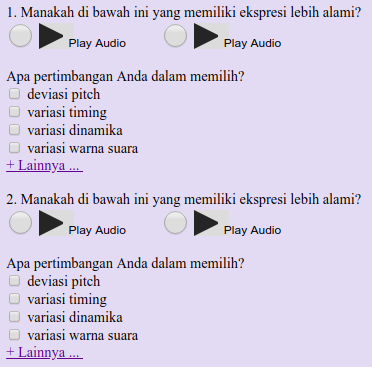
\includegraphics[width=0.8\textwidth]{resources/questionnaire_screenshot.png}
    \caption{Tampilan cuplikan kuesioner yang digunakan untuk uji preferensi kealamian}\label{fig-questionnaire-sample}
\end{figure}

Urutan pasangan segmen-segmen ini diacak, kemudian urutan segmen tiap pasang juga diacak. Untuk tiap pasang, responden diminta untuk memilih segmen audio yang lebih alami. Dari hasil ini, dapat dihitung persentase preferensi sistem ini terhadap sistem \textit{baseline}. Selain itu, responden juga dapat menyebutkan pertimbangan atau pendapat yang mempengaruhi bagaimana ia memilih segmen suara tersebut. Responden dapat memilih pendapat dari daftar yang telah ada ataupun menuliskan pendapat baru. Cuplikan kuesioner yang digunakan dapat dilihat pada Gambar \ref{fig-questionnaire-sample}. %TODO Mean Preference Score dibenerin

\section{Hasil Eksperimen Komponen Sistem}

Hasil eksperimen komponen sistem terdiri dari eksperimen model \textit{timing}, \textit{pitch} yang terdiri dari model deviasi f0, dan \textit{timbre} yang terdiri dari model frekuensi harmonik, magnitudo harmonik, serta amplop stokastik. Eksperimen tiap-tiap model terdiri dari penyetelan parameter dan pengujian.

\subsection{Hasil penyetelan parameter}

Eksperimen model \textit{timing} dimulai dengan pemilihan teknik menggunakan validasi silang. Sebagaimana tampak pada Tabel \ref{tab-timing-model-tuning-results}, tampak bahwa teknik \textit{decision tree regression} memiliki kinerja yang lebih baik daripada ANN. Analisis lebih lanjut terhadap \textit{output} ANN tersebut menunjukkan bahwa deviasi \textit{timing} yang dihasilkan ANN adalah konstan. Hal ini menunjukkan bahwa ANN tidak dapat mempelajari pola deviasi \textit{timing} pada data latih.

\begin{table}[htbp]
    \centering
    \caption{Hasil validasi silang untuk penyetelan parameter model \textit{timing}}\label{tab-timing-model-tuning-results}
    \begin{tabular}{ |l|r| } 
     \hline
     Parameter & Pearson r untuk Nada Tiap \textit{Frame} \\
     \hline 
     \multicolumn{2}{|l|}{model regresi}\\ \hline
	 ann    &-0.03684115\\ \hline
	 dt, konteks=10, kedalaman=300     & 0.09796566\\ \hline
	 \multicolumn{2}{|l|}{penyetelan jumlah not konteks fitur}\\ \hline
	 dt, konteks=20, kedalaman=300       &0.07746795\\ \hline
	 dt, konteks=10, kedalaman=300      &0.09796566\\ \hline
	 dt, konteks=5, kedalaman=300     &0.14187831\\ \hline
	 dt, konteks=3, kedalaman=300     &\textbf{0.16475536}\\ \hline
	 dt, konteks=1, kedalaman=300      &0.10598458\\ \hline
	 \multicolumn{2}{|l|}{penyetelan kedalaman pohon}\\ \hline
	 dt, konteks=3, kedalaman=25 	 &0.15163629\\\hline
	 dt, konteks=3, kedalaman=50     &0.1326507\\\hline
	 dt, konteks=3, kedalaman=100      &0.12941929\\\hline
	 dt, konteks=3, kedalaman=300     &\textbf{0.16475536}\\ \hline
	 dt, konteks=3, kedalaman=600     &0.11958923\\\hline
	 dt, konteks=3, kedalaman=1000     &0.1351192   \\  \hline
    \end{tabular}
\end{table}

Hasil penyetelan parameter jumlah not konteks fitur dan kedalaman pohon juga terdapat pada Tabel \ref{tab-timing-model-tuning-results}. Parameter terbaik diperoleh dengan 3 not konteks fitur dan kedalaman pohon 300.

Penyetelan model berikutnya adalah penyetelan model f0. Tabel \ref{tab-f0-model-tuning-results} menunjukkan hasil validasi silang untuk penyetelan parameter model f0, dengan metrik berupa koefisien korelasi Pearson dari frekuensi fundamental hasil pembangkitan terhadap frekuensi fundamental pada data. Faktor dilasi yang menghasilkan kinerja terbaik adalah $1,2,4,8,16,32,1,2,4,8,16$. Faktor dilasi ini memiliki medan reseptif terhadap output sebelum yang lebih pendek daripada faktor dilasi pada riset neural parametrik nyanyian. Adapun tingkat \textit{noise} $\lambda$ terbaik didapatkan dengan nilai $0.4$, sama dengan pada riset neural parametrik nyanyian.

Pelatihan model f0 dengan \textit{early stopping} memiliki kinerja yang sama dengan pelatihan tanpa \textit{early stopping}. Hal ini karena dengan \textit{patience} 100, \textit{early stopping} tidak menghentikan pelatihan hingga jumlah \textit{epoch} maksimal yang bernilai 300. Karenanya, tanpa \textit{early stopping} ataupun dengan \textit{early stopping}, model f0 ini tetap dilatih dengan 300 \textit{epoch}.

\begin{table}[htbp]
    \centering
    \caption{Hasil validasi silang untuk penyetelan parameter model f0}\label{tab-f0-model-tuning-results}
    \begin{tabular}{ |l|l|l|r| } 
     \hline
     \multicolumn{3}{|l|}{Parameter} & Pearson r\\
     \cline{1-3}
     faktor dilasi & $\lambda$ & \textit{patience} & F0\\
     \hline 
	1,2,4,8,16,32,64,1,2,4,8,16,32 & 0.4 &100      &0.9525\\\hline
	1,2,4,8,16,32,1,2,4,8,16 & 0.4 &100            &0.9526\\\hline
	1,2,4,8,16,32,64,1,2,4,8,16,32 & 0.01 &100     &0.9516\\\hline
	1,2,4,8,16,32,1,2,4,8,16 & 0.01 &100           &0.9507\\\hline
	1,2,4,8,16,32,1,2,4,8,16 & 0.4 &tanpa \textit{early stopping}    &0.9526\\\hline
    \end{tabular}
\end{table}

Hasil penyetelan parameter model frekuensi harmonik tampak pada Tabel \ref{tab-freq-model-tuning-results}. Faktor dilasi yang memiliki kinerja terbaik adalah $1,2,4,1,2$, sama dengan pada riset sintesis neural parametrik nyanyian. Tingkat \textit{noise} $\lambda$ terbaik adalah $0.4$, sama dengan pada riset sintesis neural parametrik nyanyian. Model yang dilatih dengan \textit{early stopping} memiliki kinerja lebih baik daripada tanpa \textit{early stopping}.

\begin{table}[htbp]
    \centering
    \caption{Hasil validasi silang untuk penyetelan parameter model frekuensi harmonik}\label{tab-freq-model-tuning-results}
    \begin{tabular}{ |l|l|l|r| } 
     \hline
     \multicolumn{3}{|l|}{Parameter} & Rata-Rata Pearson r\\
     \cline{1-3}
     faktor dilasi & $\lambda$ & \textit{patience} &Frekuensi Harmonik \\
	 \hline 
	1,2,4,1,2 & 0.4 &100           &0.9888\\\hline
	1,2,4 & 0.4 &100               &0.9874\\\hline
	1,2,4,8,1,2,4 & 0.4 &100       &0.9884\\\hline
	1,2,4,1,2 & 0.01 &100          &0.9830\\\hline
	1,2,4 & 0.01 &100              &0.9884\\\hline
	1,2,4,8,1,2,4 & 0.01 &100      &0.9864\\\hline
	1,2,4,1,2 & 0.4 &tanpa \textit{early stopping}   &0.9839\\\hline
    \end{tabular}
\end{table}

Hasil penyetelan parameter model magnitudo harmonik tampak pada Tabel \ref{tab-mag-model-tuning-results}. Faktor dilasi yang memiliki kinerja terbaik adalah $1,2,4,8,1,2,4$. Faktor dilasi ini memiliki medan reseptif terhadap output sebelum yang lebih panjang daripada faktor dilasi pada riset neural parametrik nyanyian. Hal ini menunjukkan bahwa unsur magnitudo harmonik pada sintesis alat musik gesek membutuhkan konteks yang lebih luas daripada konteks pada sintesis suara nyanyian. Tingkat \textit{noise} $\lambda$ terbaik adalah $0.4$, sama dengan pada riset sintesis neural parametrik nyanyian. Model yang dilatih dengan \textit{early stopping} memiliki kinerja lebih baik daripada tanpa \textit{early stopping}.

\begin{table}[htbp]
    \centering
    \caption{Hasil validasi silang untuk penyetelan parameter model magnitudo harmonik}\label{tab-mag-model-tuning-results}
    \begin{tabular}{ |l|l|l|r| } 
     \hline
     \multicolumn{3}{|l|}{Parameter} & Rata-Rata Pearson r\\
     \cline{1-3}
     faktor dilasi & $\lambda$ & \textit{patience} & Magnitudo Harmonik\\
	 \hline 
	1,2,4,1,2 & 0.4 &100           &0.1717\\\hline
	1,2,4,8,1,2,4 & 0.4 &100       &0.2002\\\hline
	1,2,4 & 0.4 &100               &0.0980\\\hline
	1,2,4,1,2 & 0.01 &100          &0.1338\\\hline
	1,2,4,8,1,2,4 & 0.01 &100      &0.0592\\\hline
	1,2,4 & 0.01 &100              &0.0556\\\hline
	1,2,4 & 0.4 &tanpa \textit{early stopping}       &0.1704\\\hline
    \end{tabular}
\end{table}

Hasil penyetelan parmeter model amplop stokastik tampak pada Tabel \ref{tab-stoc-model-tuning-results}. Faktor dilasi yang memiliki kinerja terbaik adalah $1,2,4,1,2$, sama dengan pada riset sintesis neural parametrik nyanyian. Tingkat \textit{noise} $\lambda$ terbaik adalah $0.4$, sama dengan pada riset sintesis neural parametrik nyanyian. Model yang dilatih dengan \textit{early stopping} memiliki kinerja lebih baik daripada tanpa \textit{early stopping}.

\begin{table}[htbp]
    \centering
    \caption{Hasil validasi silang untuk penyetelan parameter model amplop stokastik}\label{tab-stoc-model-tuning-results}
    \begin{tabular}{ |l|l|l|r| } 
     \hline
     \multicolumn{3}{|l|}{Parameter} & Rata-Rata Pearson r\\
     \cline{1-3}
     faktor dilasi & $\lambda$ & \textit{patience} & Amplop Stokastik\\
	 \hline 
	1,2,4,1,2& 0.4& 100           & 0.0391\\\hline
	1,2,4& 0.4& 100               & 0.0729\\\hline
	1,2,4,8,1,2,4& 0.4& 100       &-0.0028\\\hline
	1,2,4,1,2& 0.01& 100          &-0.0328\\\hline
	1,2,4& 0.01& 100              &-0.0884\\\hline
	1,2,4,8,1,2,4& 0.01& 100      &-0.1304\\\hline
	1,2,4& 0.4& tanpa \textit{early stopping}       & 0.0493\\\hline
    \end{tabular}
\end{table}

Dengan demikian, nilai parameter-parameter model yang telah disetel terdapat pada Tabel \ref{tab-timbre-pitch-model-parameters} dan Tabel \ref{tab-timing-model-parameters}. Nilai parameter-parameter model \textit{timing} terdapat pada Tabel \ref{tab-timing-model-parameters}. Nilai parameter-parameter model \textit{pitch} dan model timbre terdapat pada Tabel \ref{tab-timbre-pitch-model-parameters}.
\begin{table}[htbp]
	\centering
	\caption{Nilai parameter-parameter model \textit{timing}}\label{tab-timing-model-parameters}
	\begin{tabular}{|l|l|}
	\hline
	Parameter&Nilai \\\hline
	Fitur not konteks & 3 sebelum, 3 sesudah\\\hline
	Kedalaman maksimal pohon & 300\\\hline
	\end{tabular}
\end{table}


\begin{table}[htbp]
	\newlength\colwidth
	\setlength\colwidth{\dimexpr.2\columnwidth-2\tabcolsep-0.2\arrayrulewidth\relax}
	\centering
	\caption{Nilai parameter-parameter model \textit{pitch} dan model timbre}\label{tab-timbre-pitch-model-parameters}
	\begin{tabular}{|p{\colwidth}|p{\colwidth}|p{\colwidth}|p{\colwidth}|p{\colwidth}|}
	\hline
	\multirow{2}{*}{Parameter}&\multicolumn{3}{|p{\dimexpr 3\colwidth}|}{Model Timbre}&{Model Pitch}\\\cline{2-5}
	&Deviasi Frekuensi Harmonik&Magnitudo Harmonik (ternormalisasi minmax)&Amplop Stokastik (ternormalisasi minmax)&Deviasi F0 (skala: \textit{semitone})\\\hline
	Dimensi fitur&20&20&6&1\\\hline
	Input tambahan (dim.)& Deviasi F0 (1) & Deviasi F0 (1) \newline Dev. HFreq (20) & Deviasi F0 (1) \newline Dev. HFreq (20) \newline Hmag (20) & - \\
	\hline
	Not konteks input kontrol & \multicolumn{4}{|p{\dimexpr 4\colwidth}|}{
	Not sebelum dan not sesudah
	}\\\hline
	Tingkat \textit{noise} $\lambda$ & 0.4&0.4&0.4&0.4\\\hline
	Temperatur pembangkitan & 0. (harmonik terendah) – 0.0001 (harmonik tertinggi) & 0. (harmonik terendah) – 0.01 (harmonik tertinggi) & 0.001 & 0.001 \\\hline
	Konvolusi kausal awal & $10 \times 1$ & $10 \times 1$ & $10 \times 1 $ & $20 \times 1 $\\\hline
	Kanal residual & 20 & 130 & 20 & 100 \\\hline
	Konvolusi terdilasi & $2\times 1$ & $2\times 1$ & $2\times 1$ & $2\times 1$ \\\hline
	Jumlah lapisan & 5 & 7 & 3 & 11\\\hline
	Lapisan per \textit{stage} & 3 & 4 & 3 & 6\\\hline
	Faktor dilasi & 1,2,4,1,2 & 1,2,4,8,1,2,4 & 1,2,4 & 1,2,4,8,16,32, 1,2,4,8,16\\\hline
	Medan reseptif&58 ms & 93 ms & 49 ms & 33 ms\\\hline
	Kanal \textit{skip}&16&240&20&100\\\hline
	\textit{Output stage}&Tanh$\rightarrow 1\times 1 \rightarrow 20\times CGM_{K=4}$&Tanh$\rightarrow 1\times 1 \rightarrow 20\times CGM_{K=4}$&Tanh$\rightarrow 1\times 1 \rightarrow 6\times CGM_{K=4}$&Tanh$\rightarrow 1\times 1 \rightarrow 1\times CGM_{K=4}$\\\hline
	Ukuran \textit{batch} &32&32&32& 64\\\hline
	Jumlah \textit{frame} output valid & 101 & 101 & 101 & 101 \\\hline
	\textit{Learning rate} & default & default & default & default\\\hline
	Jumlah \textit{epoch} maksimal & 2000 & 2000 & 2000 & 300 \\\hline
	\textit{Patience} & 100 & 100 & 100 & 100 \\\hline
	\end{tabular}
\end{table}
\subsection{Perbandingan kinerja model dari keseluruhan data latih dengan model dari sebagian data latih}

Tabel \ref{tab-timing-model-subset-results} menunjukkan perbandingan kinerja model \textit{timing} yang dilatih dengan keseluruhan data latih dan model yang dilatih dengan sebagian data latih. Hasil ini membuktikan bahwa untuk model \textit{timing}, model yang dilatih dengan keseluruhan data latih memiliki kinerja lebih baik. Adapun model yang dilatih dengan sebagian data latih, umumnya memiliki kinerja terhadap data uji yang lebih buruk. Hal ini karena model \textit{timing} tidak mengalami anomali yang dialami oleh model-model yang menggunakan arsitektur Wavenet yang dimodifikasi.

\begin{table}[htbp]
    \centering
    \caption{Kinerja model timing dengan berbagai subset data latih}\label{tab-timing-model-subset-results}
    \begin{tabular}{ |l|r|r| } 
     \hline
     \multirow{2}{*}{Subset data latih} & \multicolumn{2}{l|}{Pearson r untuk Nada Tiap \textit{Frame}} \\
     \cline{2-3}
     & terhadap data latih & terhadap data uji \\\hline

	subset-1          &0.1816  &0.0528\\\hline
	subset-2          &0.2049 &-0.0252\\\hline
	subset-3          &0.2009  &0.1483\\\hline
	subset-4          &0.2515  &0.0187\\\hline
	subset-5          &0.2868  &0.0001\\\hline
	data latih utuh			 &0.2511  &0.2213\\\hline
    \end{tabular}
\end{table}

Tabel \ref{tab-f0-model-subset-results} menunjukkan perbandingan kinerja model f0 yang dilatih dengan keseluruhan data latih dan model yang dilatih dengan sebagian data latih. Tiap subset-$i$ adalah data latih \textit{fold}-$i$ dari \textit{fold}-\textit{fold} yang sebelumnya digunakan pada validasi silang $5$-\textit{fold}.

Perhatikan bahwa kinerja tertinggi terhadap data latih diperoleh dengan subset subset-1. Kinerja model yang dilatih dengan subset ini terhadap data uji lebih baik daripada kinerja model yang dilatih dengan keseluruhan data latih. Hal ini menunjukkan bahwa untuk model f0, dengan memilih subset data latih dengan kinerja terhadap data latih tertinggi, kinerjanya kepada data uji lebih baik daripada model yang dilatih dengan data latih utuh. 

Terdapat dua kemungkinan yang menyebabkan hal ini. Kemungkinan pertama, penambahan data latih menurunkan kinerja. Kemungkinan kedua adalah kualitas data latih tidak merata.

\begin{table}[htbp]
    \centering
    \caption{Kinerja model f0 dengan berbagai subset data latih}\label{tab-f0-model-subset-results}
    \begin{tabular}{ |l|r|r| } 
     \hline
     \multirow{2}{*}{Subset data latih} & \multicolumn{2}{l|}{Pearson r untuk F0 Tiap \textit{Frame}} \\
     \cline{2-3}
     & terhadap data latih & terhadap data uji \\\hline
	subset-1          &0.9529  & 0.9551\\\hline
	subset-2          &0.9511  &-0.9534\\\hline
	subset-3          &0.9520  &0.9534\\\hline
	subset-4          &0.9512  &0.9547\\\hline
	subset-5          &0.9513  &0.9547\\\hline
	data latih utuh			 &0.9514  &0.9547\\\hline
    \end{tabular}
\end{table}

Tabel \ref{tab-freq-model-subset-results} menunjukkan  perbandingan kinerja model frekuensi harmonik yang dilatih dengan keseluruhan data latih dan model yang dilatih dengan sebagian data latih. Perhatikan bahwa kinerja tertinggi terhadap data latih diperoleh dengan data latih utuh. Kinerja tertinggi terhadap data uji juga didapatkan dengan model yang dilatih dengan data latih utuh. 

Hal ini menunjukkan bahwa untuk model frekuensi harmonik, penambahan data latih meningkatkan kinerja model. Selain itu, ditunjukkan pula bahwa untuk model frekuensi harmonik, pemilihan kumpulan data latih berdasarkan kinera terhadap data latih utuh akan menghasilkan kinerja tertinggi terhadap data uji.

\begin{table}[htbp]
    \centering
    \caption{Kinerja model frekuensi harmonik dengan berbagai subset data latih}\label{tab-freq-model-subset-results}
    \begin{tabular}{ |l|r|r| } 
     \hline
     \multirow{2}{*}{Subset data latih} & \multicolumn{2}{l|}{Pearson r untuk Frekuensi Harmonik Tiap \textit{Frame}} \\
     \cline{2-3}
     & terhadap data latih & terhadap data uji \\\hline
	subset-1      &0.9897  &0.9924\\\hline
	subset-2      &0.9898  &0.9917\\\hline
	subset-3      &0.9909  &0.9924\\\hline
	subset-4      &0.9868  &0.9930\\\hline
	subset-5      &0.9896  &0.9932\\\hline
	data latih utuh      &0.9920  &0.9935\\\hline
    \end{tabular}
\end{table}

Tabel \ref{tab-mag-model-subset-results} menunjukkan perbandingan kinerja model magnitudo harmonik yang dilatih dengan keseluruhan data latih dan model yang dilatih dengan sebagian data latih. Perhatikan bahwa kinerja tertinggi terhadap data latih diperoleh dengan subset subset-5. Kinerja model yang dilatih dengan subset ini terhadap data uji lebih baik daripada kinerja model yang dilatih dengan keseluruhan data latih. Hal ini menunjukkan bahwa untuk model magnitudo harmonik, dengan memilih subset data latih dengan kinerja terhadap data latih tertinggi, kinerjanya kepada data uji lebih baik daripada model yang dilatih dengan data latih utuh. 

Perhatikan pula bahwa kinerja model yang dilatih dengan subset subset-1 hingga subset-5 memiliki kinerja terhadap data latih utuh yang lebih tinggi dibandingkan dengan model yang dilatih dengan data latih utuh. Begitu pula kinerja terhadap data uji dari model yang dilatih dengan subset subset-1 hingga subset-5 secara umum lebih baik daripada model yang dilatih dengan data latih utuh. Hal ini menunjukkan bahwa untuk model magnitudo harmonik, data latih yang berukuran lebih besar memiliki kinerja lebih rendah.

\begin{table}[htbp]
    \centering
    \caption{Kinerja model magnitudo harmonik dengan berbagai subset data latih}\label{tab-mag-model-subset-results}
    \begin{tabular}{ |l|r|r| } 
     \hline
     \multirow{2}{*}{Subset data latih} & \multicolumn{2}{l|}{Pearson r untuk Magnitudo Harmonik Tiap \textit{Frame}} \\
     \cline{2-3}
     & terhadap data latih & terhadap data uji \\\hline
	subset-1      &0.3997  &0.3031\\\hline
	subset-2      &0.3846  &0.2725\\\hline
	subset-3      &0.4118  &0.2469\\\hline
	subset-4      &0.3886  &0.2972\\\hline
	subset-5      &0.4469  &0.3211\\\hline
	data latih utuh    	 &0.3050  &0.2534\\\hline
    \end{tabular}
\end{table}

\begin{figure}[htbp]
    \centering
    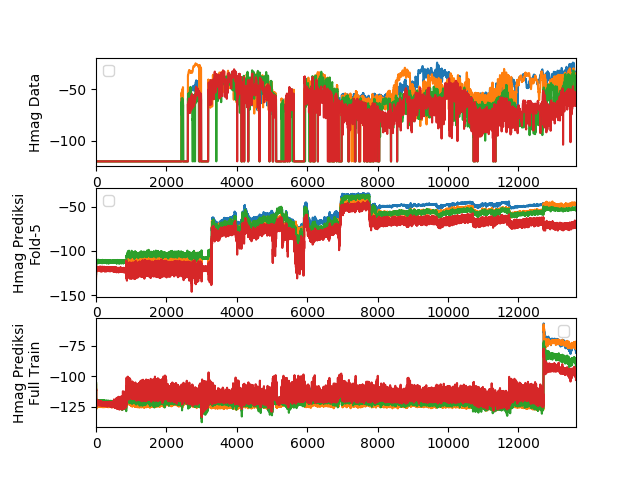
\includegraphics[width=0.8\textwidth]{resources/Analisis_Hmag_subset.png}
    \caption{Contoh perbandingan keluaran model magnitudo harmonik yang dilatih dengan subset dan keseluruhan data latih (4 harmonik pertama), dengan masukan \textit{timing}, f0, dan hfreq dari dataset}\label{fig-hmag-subset-output-sample}
\end{figure}

Gambar \ref{fig-hmag-subset-output-sample} menujukkan contoh perbandingan keluaran model magnitudo harmonik yang dilatih dengan subset dan yang dilatih dengan keseluruhan data latih. Grafik paling atas menunjukkan referensi pada data, grafik tengah menunjukkan keluaran dari model yang dilatih dengan subset subset-5, dan grafik paling bawah menunjukkan keluaran dari model yang dilatih dengan keseluruhan data latih. Tampak bahwa model yang dilatih dengan keseluruhan data latih lebih banyak menghasilkan magnitudo kecil. Pada taraf magnitudo -100 hingga -120 dB seperti pada gambar tersebut, pendengar akan mendengar seolah-olah tidak ada suara.

Tabel \ref{tab-stoc-model-subset-results} menunjukkan perbandingan kinerja model stokastik yang dilatih dengan keseluruhan data latih dan model yang dilatih dengan sebagian data latih. Perhatikan bahwa kinerja tertinggi terhadap data latih diperoleh dengan subset subset-1. Kinerja model yang dilatih dengan subset ini terhadap data uji lebih baik daripada kinerja model yang dilatih dengan keseluruhan data latih. Hal ini menunjukkan bahwa untuk model stokastik, dengan memilih subset data latih dengan kinerja terhadap data latih tertinggi, kinerjanya kepada data uji lebih baik daripada model yang dilatih dengan data latih utuh. 

Terdapat dua kemungkinan yang menyebabkan hal ini. Kemungkinan pertama, penambahan data latih menurunkan kinerja. Kemungkinan kedua adalah kualitas data latih tidak merata.

\begin{table}[htbp]
    \centering
    \caption{Kinerja model amplop stokastik dengan berbagai subset data latih}\label{tab-stoc-model-subset-results}
    \begin{tabular}{ |l|r|r| } 
     \hline
     \multirow{2}{*}{Subset data latih} & \multicolumn{2}{l|}{Pearson r untuk Amplop Stokastik Tiap \textit{Frame}} \\
     \cline{2-3}
     & terhadap data latih & terhadap data uji \\\hline
	subset-1       &0.2471  &0.0211\\\hline
	subset-2       &0.5555  &0.0508\\\hline
	subset-3       &0.2820  &0.0355\\\hline
	subset-4       &0.5925  &0.0640\\\hline
	subset-5       &0.5598  &0.1240\\\hline
	data latih utuh       &0.4303  &0.0552\\\hline
    \end{tabular}
\end{table}

Dengan demikian, dapat diambil kesimpulan untuk skema pemilihan subset. Untuk model \textit{timing}, kinerja model yang dilatih dengan keseluruhan dataset lebih besar daripada model yang dilatih dengan subset yang dipilih dengan skema tersebut. Untuk model frekuensi harmonik, dari skema pemilihan tersebut dipilih data latih utuh, sehingga kinerja dengan skema tersebut sama dengan apabila model dilatih tanpa skema pemilihan subset data latih. Untuk model f0, magnitudo harmonik, dan amplop stokastik, model yang dilatih dengan dataset yang dipilih dengan skema pemilihan subset menghasilkan kinerja yang lebih baik daripada model yang dilatih dengan data latih utuh.

Dengan demikian, pernyataan pada riset neural parametrik nyanyian bahwa penambahan data latih dapat menurunkan kinerja. Untuk jaringan syaraf tiruan dengan arsitektur Wavenet yang dimodifikasi, penambahan data latih dapat menurunkan kinerja. Adapun untuk model \textit{timing} yang tidak menggunakan arsitektur tersebut, penambahan data latih tetap meningkatkan kinerja.

\subsection{Hasil Uji Korelasi Tiap Komponen}

Tabel \ref{tab-timing-testing-results} menunjukkan korelasi nada tiap-tiap \textit{frame} dengan \textit{timing} not keluaran model \textit{timing}. Korelasi ini diukur terhadap nada tiap-tiap \textit{frame} dengan \textit{timing} ekspresif pada data. Nilai koefisien korelasi di atas 0 menunjukkan bahwa model berhasil mempelajari pola \textit{timing}. Namun, koefisien korelasi ini masih bernilai rendah. Kinerja model ini rendah baik terhadap data latih maupun data uji. Hal ini menunjukkan adanya \textit{underfitting}.

\begin{table}[htbp]
    \centering
    \caption{Hasil uji korelasi model timing}\label{tab-timing-testing-results}
    \begin{tabular}{ |l|r|r| } 
     \cline{2-3}
     \multicolumn{1}{l|}{}&Terhadap data latih&Terhadap data uji\\\hline
	 Pearson r&0.2511  &0.2213\\\hline
    \end{tabular}
\end{table}
%TODO analisis hasil eksperimen model timing

Tabel \ref{tab-f0-testing-results} menunjukkan koefisien korelasi f0 tiap-tiap \textit{frame} keluaran model f0 terhadap f0 pada data. Nilai koefisien korelasi di atas 0 menunjukkan bahwa model berhasil mempelajari pola f0. Koefisien korelasi model ini tidak mencapai nilai 1, namun sudah mencapai 0.9550 terhadap data uji. Tidak terjadi \textit{overfitting} di sini.
\begin{table}[htbp]
    \centering
    \caption{Hasil uji korelasi model f0}\label{tab-f0-testing-results}
    \begin{tabular}{ |l|r|r| } 
     \cline{2-3}
     \multicolumn{1}{l|}{}&Terhadap data latih&Terhadap data uji\\\hline
	 Pearson r&0.9529  &0.9550\\\hline
    \end{tabular}
\end{table}

\begin{figure}[h]
    \centering
    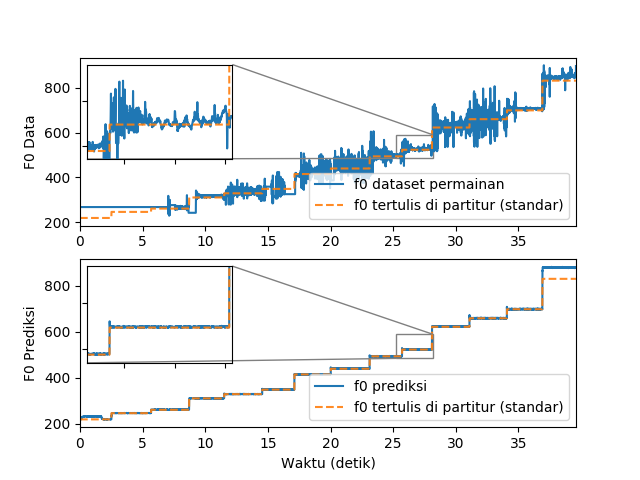
\includegraphics[width=0.8\textwidth]{resources/Analisis_F0.png}
    \caption{Contoh keluaran model f0, dengan masukan \textit{timing} dari dataset}\label{fig-f0-output-sample}
\end{figure}

Kekurangan yang masih terjadi di model f0 adalah menganggap perubahan jangka-pendek dari f0 sebagai \textit{noise} dan hanya dirata-ratakan oleh model. Hal ini tampak pada contoh keluaran model f0 pada Gambar \ref{fig-f0-output-sample}. Pada bagian atas terlihat contoh f0 dari dataset, sedangkan pada bagian bawah terlihat f0 prediksi untuk sampel tersebut. Pada kedua bagian tersebut, terdapat bagian yang diperbesar untuk melihat perubahan jangka-pendek f0 tersebut. 

Pada bagian yang diperbesar pada gambar tersebut, terlihat dua jenis perubahan jangka-pendek f0 yang dianggap sebagai \textit{noise} oleh model. Pada bagian kiri, terlihat \textit{spike} pada data dianggap sebagai \textit{noise} oleh model, dan pada f0 prediksi hal tersebut hilang. Pada bagian kanan dari perbesaran tersebut pada f0 dari data, terlihat pola osilasi yang menunukkan \textit{vibrato}. Pada f0 prediksi hal tersebut hilang dan dirata-ratakan.

Tabel \ref{tab-freq-testing-results} menunjukkan koefisien korelasi frekuensi harmonik tiap-tiap \textit{frame} keluaran model frekuensi harmonik terhadap frekuensi harmonik pada data. Nilai koefisien korelasi di atas 0 menunjukkan bahwa model berhasil mempelajari pola frekuensi harmonik. Koefisien korelasi model ini tidak mencapai nilai 1, namun sudah mencapai 0.9550 terhadap data uji. Tidak terjadi \textit{overfitting} di sini.
\begin{table}[htbp]
    \centering
    \caption{Hasil uji korelasi model frekuensi harmonik}\label{tab-freq-testing-results}
    \begin{tabular}{ |l|r|r| } 
     \cline{2-3}
     \multicolumn{1}{l|}{}&Terhadap data latih&Terhadap data uji\\\hline
	 Pearson r&0.9920  &0.9935\\\hline
    \end{tabular}
\end{table}

\begin{figure}[h]
    \centering
    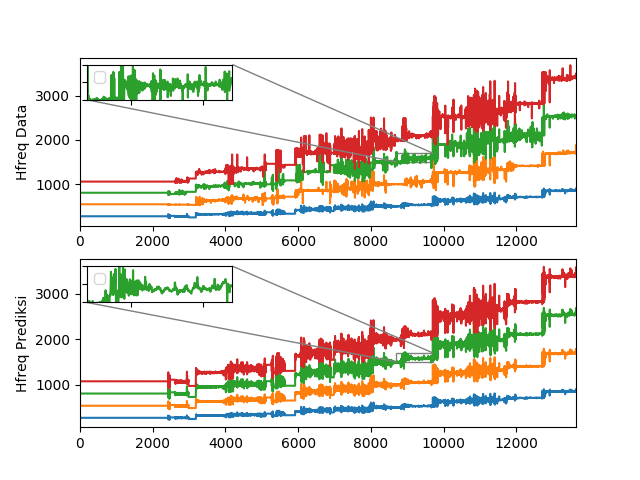
\includegraphics[width=0.8\textwidth]{resources/Analisis_Hfreq.png}
    \caption{Contoh keluaran model frekuensi harmonik (4 harmonik pertama), dengan masukan \textit{timing} dan f0 dari dataset}\label{fig-hfreq-output-sample}
\end{figure}

Kekurangan yang masih terjadi di model frekuensi harmonik adalah menganggap perubahan jangka-pendek dari frekuensi harmonik sebagai \textit{noise} dan hanya dirata-ratakan oleh model. Hal ini tampak pada contoh keluaran model frekuensi harmonik pada Gambar \ref{fig-hfreq-output-sample}. Pada bagian atas terlihat contoh frekuensi harmonik dari dataset, sedangkan pada bagian bawah terlihat frekuensi harmonik prediksi untuk sampel tersebut. Pada kedua bagian tersebut, terdapat bagian yang diperbesar untuk melihat perubahan jangka-pendek frekuensi harmonik tersebut. 

Pada bagian yang diperbesar pada gambar tersebut, terlihat bahwa pola \textit{spike} dari deviasi frekuensi harmonik hilang, dan hanya dirata-ratakan saja. Padahal, pada dataset, untuk harmonik tinggi, terdapat pola seperti \textit{spike}. Adapun \textit{vibrato} dan \textit{spike} dari f0, bila ada, diteruskan ke harmonik selanjutnya, tanpa deviasi.

Tabel \ref{tab-mag-testing-results} menunjukkan koefisien korelasi magnitudo harmonik tiap-tiap \textit{frame} keluaran model magnitudo harmonik terhadap magnitudo harmonik pada data. Nilai koefisien korelasi di atas 0 menunjukkan bahwa model berhasil mempelajari pola magnitudo harmonik. Namun, koefisien korelasi ini masih bernilai rendah. Kinerja model ini rendah baik terhadap data latih maupun data uji. Hal ini menunjukkan adanya \textit{underfitting}.

\begin{table}[htbp]
    \centering
    \caption{Hasil uji korelasi model magnitudo harmonik}\label{tab-mag-testing-results}
    \begin{tabular}{ |l|r|r| } 
     \cline{2-3}
     \multicolumn{1}{l|}{}&Terhadap data latih&Terhadap data uji\\\hline
	 Pearson r&0.4469  &0.3211\\\hline
    \end{tabular}
\end{table}

\begin{figure}[htbp]
    \centering
    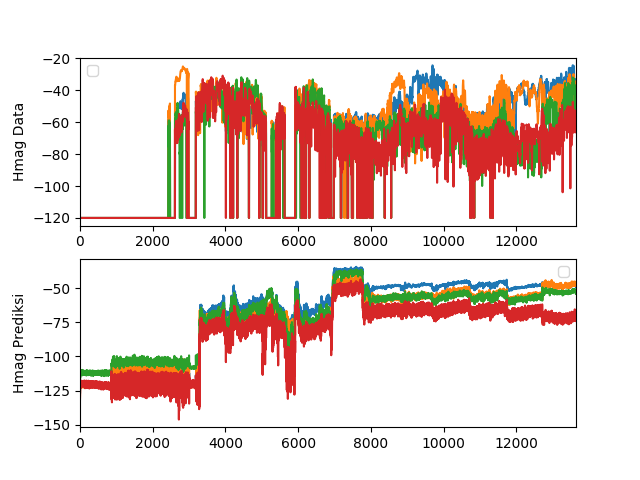
\includegraphics[width=0.8\textwidth]{resources/Analisis_Hmag.png}
    \caption{Contoh keluaran model magnitudo harmonik (4 harmonik pertama), dengan masukan \textit{timing}, f0, dan hfreq dari dataset}\label{fig-hmag-output-sample}
\end{figure}

\begin{figure}[htbp]
    \centering
    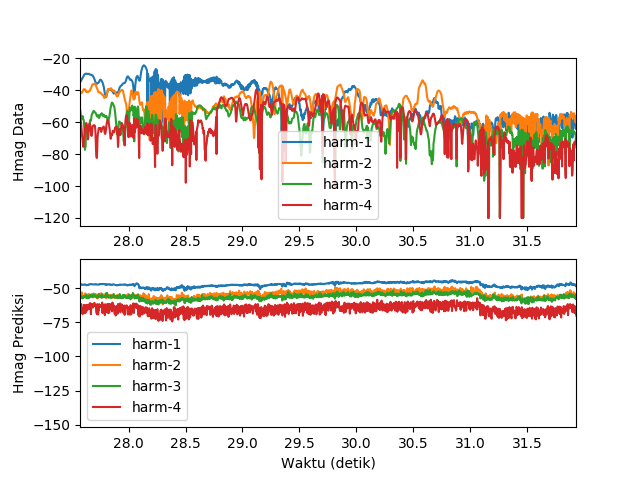
\includegraphics[width=0.8\textwidth]{resources/Analisis_Hmag_zoomed.png}
    \caption{(Diperbesar ke satu not) Contoh keluaran model magnitudo harmonik (4 harmonik pertama), dengan masukan \textit{timing}, f0, dan hfreq dari dataset}\label{fig-hmag-output-sample-zoomed}
\end{figure}

Kekurangan yang masih terjadi di model magnitudo harmonik adalah menganggap perubahan jangka-pendek dari magnitudo harmonik sebagai \textit{noise} dan hanya dirata-ratakan oleh model. Hal ini tampak pada contoh keluaran model magnitudo harmonik pada Gambar \ref{fig-hmag-output-sample}. Pada bagian atas terlihat contoh magnitudo harmonik dari dataset, sedangkan pada bagian bawah terlihat magnitudo harmonik prediksi untuk sampel tersebut. Tampilan yang diperbesar tampak pada Gambar \ref{fig-hmag-output-sample-zoomed}.

Tampak bahwa model ini mampu membangkitkan ekspresi naik turunnya magnitudo secara umum. Namun, pola jangka-pendek yang dihasilkan berbeda dengan dataset. Terdapat beberapa perbedaan antara magnitudo harmonik pada dataset dan magnitudo harmonik yang dibangkitkan dengan model:

\begin{itemize}
	\item magnitudo harmonik pada dataset saling menyeberangi satu sama lain, sedangkan magnitudo harmonik bangkitan berurutan
	\item magnitudo harmonik pada dataset memiliki pola \textit{spike} yang jarang namun besar, sedangkan magnitudo harmonik bangkitan memiliki \textit{noise} yang kecil namun ada di semua tempat
	\item magnitudo harmonik pada dataset memiliki bukit-bukit/punuk-punuk sedangkan magnitudo harmonik bangkitan tidak memilikinya
	\item magnitudo harmonik pada dataset memiliki bentuk yang berbeda pada transisi not, sedangkan magnitudo harmonik bangkitan memiliki bentuk yang serupa sepanjang not
\end{itemize}

Perbedaan-perbedaan ini terjadi karena model tidak cukup kompleks untuk menangkap pola detil jangka-pendek dari magnitudo harmonik dataset. Alih-alih mendapatkan pola magnitudo harmonik yang saling menyeberangi satu sama lain, model hanya menangkap pola umum rata-rata rasio magnitudo antar harmonik. Bentuk bukit-bukit/punuk-punuk dan \textit{spike} yang jarang ditangkap sebagai \textit{noise} yang direpresentasikan dengan nilai variansi pada keluaran CGM.

Model ini juga tidak mampu memisahkan antara transisi not, awal not, akhir not, dan pertengahan not dari sisi bentuk. Ia hanya mampu mempelajari pola naik turun magnitudo secara umum. Pada hasil uji persepsi kealamian, akan tampak apakah perbedaan bentuk ini mempengaruhi persepsi kealamian.

Tabel \ref{tab-stoc-testing-results} menunjukkan koefisien korelasi amplop stokastik tiap-tiap \textit{frame} keluaran model amplop stokastik terhadap amplop stokastik pada data. Nilai koefisien korelasi di atas 0 menunjukkan bahwa model berhasil mempelajari pola amplop stokastik. Namun, koefisien korelasi ini masih bernilai rendah. Kinerja model ini rendah baik terhadap data latih maupun data uji. Namun, kinerja terhadap data uji jauh lebih rendah daripada kinerja terhadap data latih. Hal ini menunjukkan bahwa baik galat pelatihan maupun galat generalisasi pada model ini masih sangat tinggi.

\begin{table}[htbp]
    \centering
    \caption{Hasil uji korelasi model amplop stokastik}\label{tab-stoc-testing-results}
    \begin{tabular}{ |l|r|r| } 
     \cline{2-3}
     \multicolumn{1}{l|}{}&Terhadap data latih&Terhadap data uji\\\hline
	 Pearson r&0.5925  &0.0640\\\hline
    \end{tabular}
\end{table}

\begin{figure}[htbp]
    \centering
    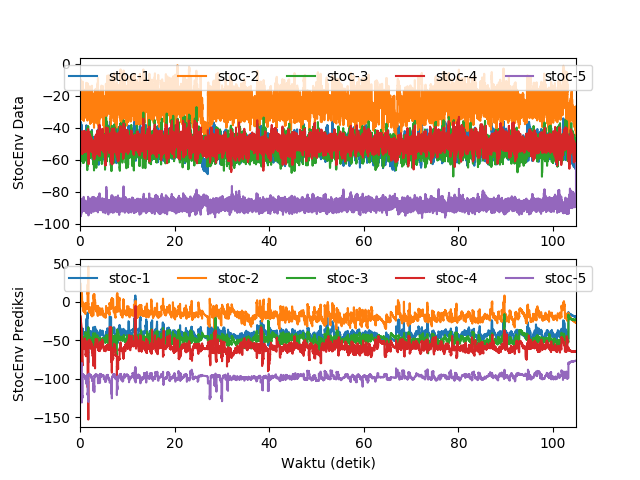
\includegraphics[width=0.8\textwidth]{resources/Analisis_StocEnv.png}
    \caption{Contoh keluaran model amplop stokastik, dengan masukan \textit{timing}, f0, dan hfreq dari dataset}\label{fig-stocenv-output-sample}
\end{figure}

\begin{figure}[htbp]
    \centering
    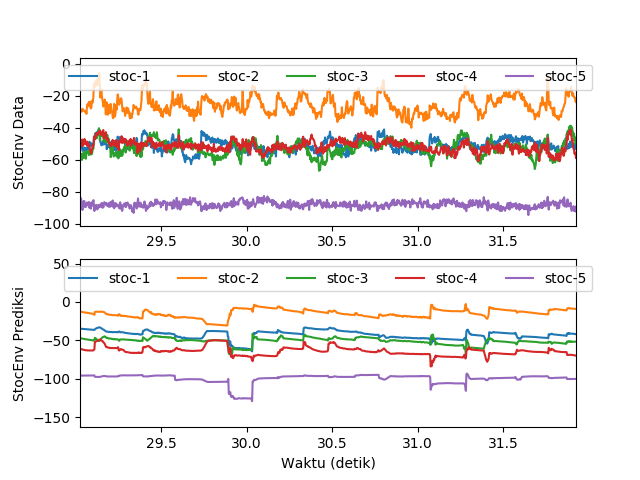
\includegraphics[width=0.8\textwidth]{resources/Analisis_StocEnv_zoomed.png}
    \caption{(Diperbesar) Contoh keluaran model amplop stokastik, dengan masukan \textit{timing}, f0, dan hfreq dari dataset}\label{fig-stocenv-output-sample-zoomed}
\end{figure}

Kekurangan yang masih terjadi di model amplop stokastik adalah menganggap perubahan jangka-pendek dari amplop stokastik sebagai \textit{noise} dan hanya dirata-ratakan oleh model. Hal ini tampak pada contoh keluaran model amplop stokastik pada Gambar \ref{fig-stocenv-output-sample}. Pada bagian atas terlihat contoh amplop stokastik dari dataset, sedangkan pada bagian bawah terlihat amplop stokastik prediksi untuk sampel tersebut. Tampilan yang diperbesar tampak pada Gambar \ref{fig-stocenv-output-sample-zoomed}.

Terdapat perbedaan antara amplop stokastik data dan amplop stokastik bangkitan:

\begin{itemize}
	\item Amplop stokastik data memiliki naik-turun dan \textit{spike} yang lebih besar
	\item Pada beberapa bagian, perubahan amplop stokastik bangkitan terbalik apabila dibandingkan dengan data
\end{itemize}

Amplop stokastik bangkitan memiliki naik-turun dan \textit{spike} yang kurang besar karena sebagian besar naik turun dan \textit{spike} tersebut dianggap sebagai \textit{noise} oleh model. Jaringan syaraf tiruan yang digunakan kemudian merata-ratakannya dan merepresentasikan perubahannya dalam keluaran variansi CGM, yang kemudian dikurangi dengan parameter temperatur.

Pada beberapa bagian, perubahan amplop stokastik bangkitan terbalik apabila dibandingkan dengan data. Di sebagian tempat, besaran amplop stokastik bangkitan turun padahal amplop stokastik pada data naik. Begitu pula sebaliknya, amplop stokastik bangkitan naik padahal amplop stokastik pada data turun. %TODO kenapa? kapan ia terbalik?

%TODO perbandingan hasil,
%TODO pola-pola yang tidak tertangkap oleh koefisien korelasi
%bahwa RPM mungkin saja memiliki nilai lebih tinggi dalam uji persepsi kealamian

\section{Hasil Uji Korelasi Sistem Utuh} \label{section-wholesystem-corrcoef-test}
Tabel \ref{tab-system-testing-results} menunjukkan hasil uji korelasi sistem DT-Neural Parametrik dan perbandingannya dengan sistem \textit{baseline} yaitu RPM. Sistem DT-Neural Parametrik berhasil mencapai koefisien korelasi di atas nol, yang artinya sistem ini berhasil mempelajari sebagian pola-pola ekspresi. Namun, nilai koefisien korelasi ini masih rendah, artinya tidak semua pola-pola ekspresi berhasil dipelajari dengan benar.

\begin{table}[htbp]
    \centering
    \caption{Hasil pengujian korelasi sistem utuh}\label{tab-system-testing-results}
    \begin{tabular}{ |l|r|r| } 
     \cline{2-3}
     \multicolumn{1}{l|}{}&\multicolumn{2}{|l|}{Rata-Rata Pearson r Semua Komponen}\\\hline
     Sistem&Terhadap data latih&Terhadap data uji\\\hline
	 RPM&-0.2380* &-0.0020\\\hline
	 DT-Neural Parametrik& 0.1188**&0.1133\\\hline
	 \multicolumn{3}{l}{*RPM tidak dilatih dengan data latih ini}\\
	 \multicolumn{3}{l}{**Model komponen dilatih dengan subset yang telah dipilih}\\
    \end{tabular}
\end{table}

Nilai koefisien korelasi yang dicapai oleh sistem ini lebih tinggi daripada sistem RPM. Sistem yang diajukan menghasilkan keluaran dengan koefisien korelasi 0.1188 terhadap data latih, sementara RPM hanya menghasilkan -0.2380, dengan catatan bahwa sistem RPM memang tidak dilatih menggunakan data latih ini. Untuk membandingkan kinerja generalisasi kedua sistem, dibandingkan kinerjanya terhadap data uji. Sistem yang diajukan menghasilkan koefisien korelasi 0.1133 terhadap data uji, sementara sistem RPM hanya menghasilkan koefisien korelasi -0.0020.

\begin{figure}[htbp]
    \centering
    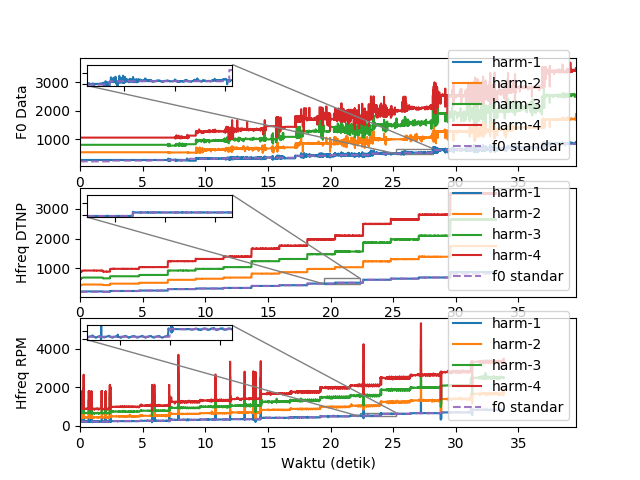
\includegraphics[width=0.8\textwidth]{resources/Analisis_wholesystem_Hfreq.png}
    \caption{Contoh frekuensi harmonik (4 harmonik pertama) yang dihasilkan oleh sistem DT-Neural Parametrik utuh dan RPM}\label{fig-wholesystem-hfreq-output-sample}
\end{figure}

Gambar \ref{fig-wholesystem-hfreq-output-sample} menunjukkan contoh frekuensi harmonik keluaran sistem Neural Parametrik dan keluaran \textit{baseline} RPM. Untuk pola jangka-pendek, teknik RPM tampak lebih mirip Tampak bahwa keluaran \textit{baseline} RPM memiliki pola osilasi (\textit{vibrato}) pada frekuensi fundamental dan keluaran teknik Neural Parametrik tidak memiliki pola osilasi (\textit{vibrato}). Pola \textit{spike} frekuensi fundamental tidak ada di keluaran kedua sistem. Begitu pula variasi keluaran frekuensi harmonik tidak ada di keluaran kedua sistem. Pola jangka-pendek ini tidak tertangkap oleh metrik koefisien korelasi.

Untuk pola-pola jangka-panjang, teknik Neural Parametrik mampu menghasilkan deviasi \textit{pitch} yang mirip dengan deviasi \textit{pitch} pada dataset. Pada contoh pada Gambar \ref{fig-wholesystem-hfreq-output-sample}, pada awal-awal permainan, frekuensi fundamental dari audio yang dihasilkan oleh teknik Neural Parametrik lebih tinggi daripada frekuensi fundamental standar untuk not yang sedang dimainkan. Pada dataset, frekuensi fundamental dari audio lebih tinggi daripada frekuensi fundamental standar. Adapun pada keluaran sistem RPM, frekuensi fundamental yang dihasilkan sama dengan frekuensi fundamental standar. Pola jangka-panjang inilah yang tertangkap oleh koefisien korelasi.

\begin{figure}[htbp]
    \centering
    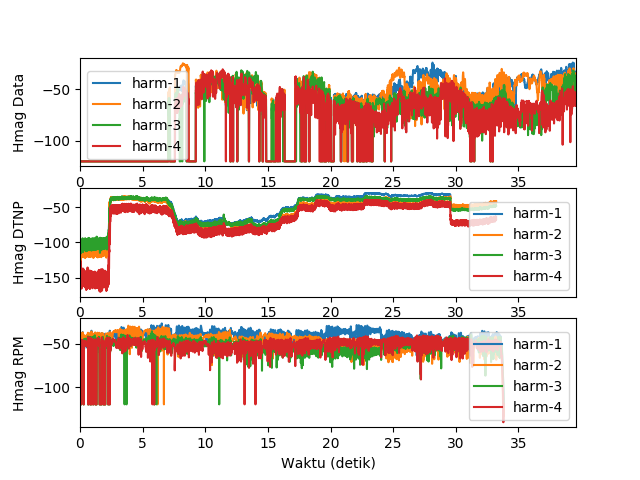
\includegraphics[width=0.8\textwidth]{resources/Analisis_wholesystem_Hmag.png}
    \caption{Contoh magnitudo harmonik (4 harmonik pertama) yang dihasilkan oleh sistem DT-Neural Parametrik utuh dan RPM}\label{fig-wholesystem-hmag-output-sample}
\end{figure}

\begin{figure}[htbp]
    \centering
    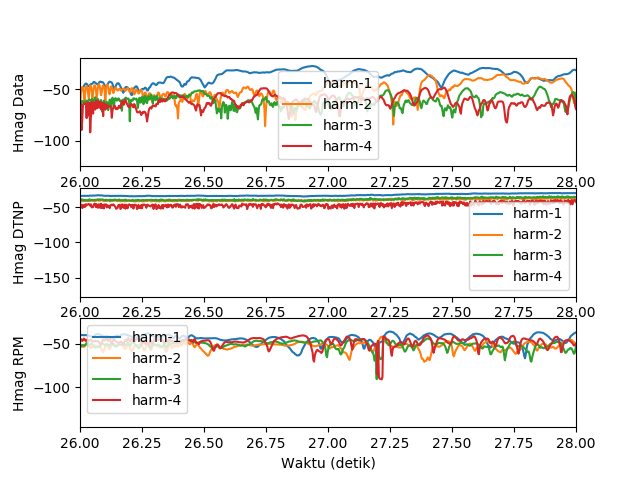
\includegraphics[width=0.8\textwidth]{resources/Analisis_wholesystem_Hmag_zoomed.png}
    \caption{(Diperbesar) Contoh magnitudo harmonik (4 harmonik pertama) yang dihasilkan oleh sistem DT-Neural Parametrik utuh dan RPM}\label{fig-wholesystem-hmag-output-sample-zoomed}
\end{figure}

Gambar \ref{fig-wholesystem-hmag-output-sample} menunjukkan contoh magnitudo harmonik keluaran sistem Neural Parametrik dan keluaran \textit{baseline} RPM. Gambar \ref{fig-wholesystem-hmag-output-sample-zoomed} menunjukkan versi yang diperbesar. Magnitudo harmonik keluaran sistem Neural Parametrik memiliki variasi jangka-panjang secara umum. Namun, untuk variasi jangka-pendek seperti pola bukit-bukit, punuk-punuk, serta saling menyilang antar harmonik, teknik Neural Parametrik tidak mampu menangkapnya. Berbeda dengan itu, magnitudo harmonik RPM tidak memiliki pola jangka-panjang. RPM mampu menghasilkan pola jangka-pendek seperti pola bukit-bukit, punuk-punuk, serta saling menyilang antar harmonik, namun tetap terdapat perbedaan dengan pola pada dataset. Bukit-bukit dan punuk-punuk pada magnitudo harmonik dataset memiliki kerapatan yang bermacam-macam, adapun pada keluaran RPM kerapatan bukit-bukit dan punuk-punuk ini tidak bermacam-macam.

Dengan demikian, dapat dikatakan bahwa model magnitudo harmonik pada sistem Neural Parametrik mampu menangkap pola keras-lemah suara jangka-panjang. Ini yang menyebabkan koefisien korelasinya lebih tinggi daripada RPM. Pada pola jangka-panjang, RPM tidak memiliki variasi keras-lemah suara. Pada pola jangka-pendek, bentuk bukit-bukit serta kerapatannya pada keluaran RPM berbeda dengan pada dataset. Karenanya, kemiripannya tidak tertangkap pada koefisien korelasi. Untuk pola jangka-pendek, meski tidak tertangkap pada koefisien korelasi, terlihat bahwa RPM memiliki kemiripan dengan dataset sedangkan keluaran Neural Parametrik tidak.

\begin{figure}[htbp]
    \centering
    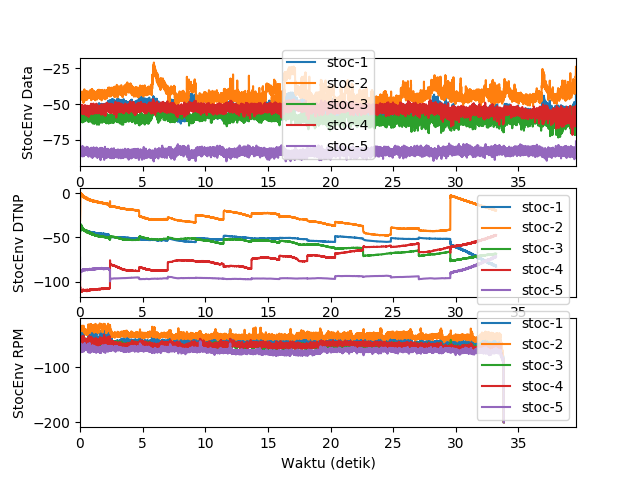
\includegraphics[width=0.8\textwidth]{resources/Analisis_wholesystem_StocEnv.png}
    \caption{Contoh amplop stokastik yang dihasilkan oleh sistem DT-Neural Parametrik utuh dan RPM}\label{fig-wholesystem-stocenv-output-sample}
\end{figure}

\begin{figure}[htbp]
    \centering
    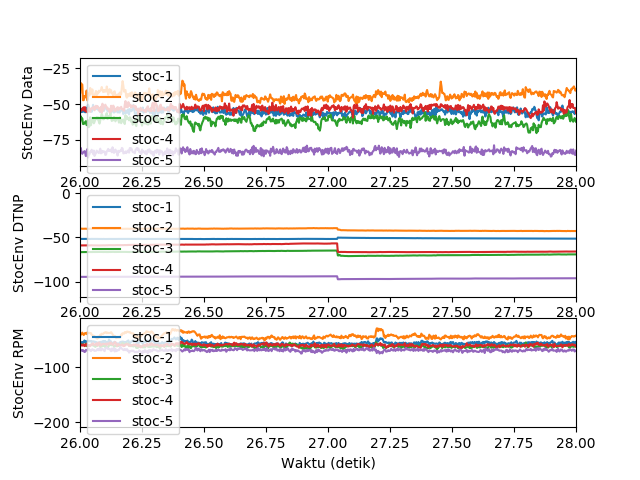
\includegraphics[width=0.8\textwidth]{resources/Analisis_wholesystem_StocEnv_zoomed.png}
    \caption{(Diperbesar) Contoh amplop stokastik yang dihasilkan oleh sistem DT-Neural Parametrik utuh dan RPM}\label{fig-wholesystem-stocenv-output-sample-zoomed}
\end{figure}

Gambar \ref{fig-wholesystem-stocenv-output-sample} menunjukkan contoh amplop stokastik keluaran sistem Neural Parametrik dan keluaran \textit{baseline} RPM. Gambar \ref{fig-wholesystem-stocenv-output-sample-zoomed} menunjukkan versi yang diperbesar. Amplop stokastik keluaran sistem Neural Parametrik memiliki variasi jangka-panjang secara umum. Namun, untuk variasi jangka-pendek, teknik Neural Parametrik tidak mampu menangkapnya. Berbeda dengan itu, amplop stokastik RPM tidak memiliki pola jangka-panjang. RPM mampu menghasilkan pola jangka-pendek, namun tetap terdapat perbedaan dengan pola pada dataset.

Selain pola jangka-pendek, kekurangan lainnya dari teknik Neural Parametrik adalah \textit{range} dari output yang dihasilkan. Teknik Neural Parametrik menghasilkan amplop stokastik dengan \textit{range} mencapai 0dB, sementara pada dataset hanya mencapai -25dB. Akibatnya, suara yang dihasilkan akan terdengar memiliki \textit{noise} berlebih. Adapun teknik RPM tidak menghasilkan nilai amplop stokastik terlalu tinggi, sehingga suaranya akan terdengar lebih bersih.

\section{Hasil Uji Preferensi Kealamian}

\begin{figure}[htbp]
  \begin{center}
  	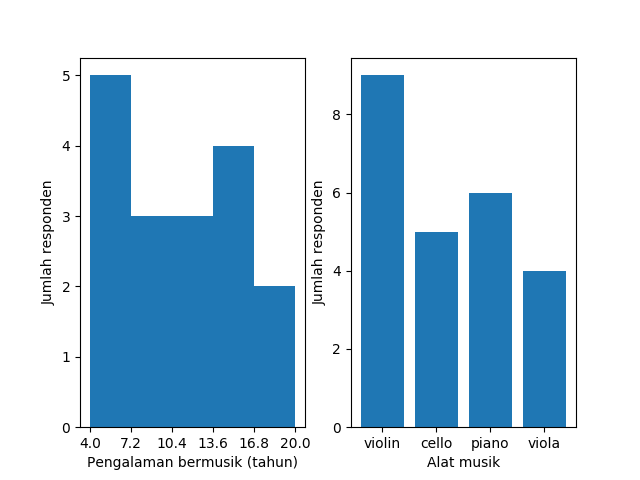
\includegraphics[width=0.8\textwidth]{resources/Karakter_responden.png}
    \caption{Karakteristik responden uji preferensi kealamian}
    \label{tab-respondent-characteristics}
  \end{center}
\end{figure}

Uji pendengar telah dilakukan kepada 17 pendengar dari kalangan pemain musik. Gambar \ref{tab-respondent-characteristics} menunjukkan pengalaman dan alat musik yang digunakan. Responden memiliki pengalaman bermain musik dengan rentang 4 s.d. 20 tahun. Semua pemain musik yang mengisi adalah pemain alat musik gesek. Beberapa di antara pemain alat musik gesek tersebut juga merupakan pemain alat musik selain alat musik gesek yaitu piano.

Karena untuk tiap pasangan teknik tiap pendengar memilih di antara 9 pasang segmen suara, maka untuk tiap pasangan teknik total terdapat 153 datum preferensi kealamian. Untuk pasangan teknik DT-Neural Parametrik dan RPM terdapat 153 datum preferensi kealamian dan untuk pasangan teknik Gabungan dan RPM terdapat 153 datum preferensi kealamian. Total ukuran data preferensi kealamian kedua pasang teknik tersebut adalah sebesar 306.

Tabel \ref{tab-preference} menunjukkan hasil uji preferensi kealamian sistem yang diajukan. Sistem neural parametrik partitur-ke-suara memiliki nilai preferensi kealamian $19,44\%$. Nilai ini kurang dari $50\%$. Artinya, oleh persepsi pendengar, sistem ini dinilai kurang alami dibandingkan dengan sistem \textit{baseline}. Begitu pula sistem gabungan yang menggunakan teknik neural parametrik sebagai perencana gestur ekspresi memiliki nilai preferensi kealamian $31,25\%$. Meskipun nilai ini lebih tinggi bila dibandingkan dengan sistem neural parametrik partitur-ke-suara, nilai ini masih kurang dari $50\%$. Artinya, oleh persepsi pendengar, suara yang dihasilkan oleh sistem ini dinilai kurang alami juga dibandingkan dengan sistem \textit{baseline}.

\begin{table}[htbp] %TODO update data
  \begin{center}
    \caption{Hasil uji preferensi kealamian dari sistem neural parametrik dan sistem gabungan}
    \label{tab-preference}
    \begin{tabular}{|l|r|r|}
    \hline
	Sistem&Jumlah Data Respon&Preferensi terhadap RPM$\pm$MoE(95$\%$ Confidence)\\
	\hline
	dtnp&	153&	$18,95\%\pm13,53\%$\\\hline
	hybrid&	153&	$29,41\%\pm22,77\%$\\\hline
	\end{tabular}
  \end{center}
\end{table}

Tabel pada Lampiran \ref{appendix-pendapat} menunjukkan pendapat-pendapat responden dalam memilih segmen yang lebih alami. Untuk tiap isi pendapat pada tabel tersebut, ditunjukkan seberapa sering pendapat tersebut muncul. Ditunjukkan seberapa sering muncul secara total dan tiap pasangan segmen. Untuk tiap pasangan segmen suara, dituliskan jumlah kemunculan pendapat tersebut berbarengan dengan terpilihnya segmen suara dari tiap teknik.

Jawaban-jawaban pendapat yang diberikan oleh responden digunakan untuk mencari penyebab-penyebab rendahnya nilai preferensi persepsi kealamian dari sistem neural parametrik dan juga sistem gabungan. Karena data ini masih berupa kemunculan pendapat-pendapat yang bermacam-macam pada data preferensi tertentu, data ini tidak dapat secara langsung menunjukkan pada teknik mana fenomena yang disebutkan terjadi, dan apakah fenomena tersebut menyebabkan terdengar lebih alami atau sebaliknya.

Untuk melihat keterhubungan antara pendapat responden dan persepsi kealamiannya, digunakan \textit{odds ratio}. \textit{Odds ratio} adalah ukuran yang menggambarkan keterhubungan antara suatu paparan dan kejadian. \textit{Odds ratio} dinyatakan sebagai rasio antara peluang kejadian dengan paparan dan peluang kejadian tanpa paparan. \parencite{oddsratio}

Dalam konteks preferensi kealamian, kejadian yang menjadi perhatian adalah ketika sistem yang diajukan dipilih. Paparan yang menjadi perhatian adalah pendapat responden. Sehingga, \textit{odds ratio} di sini adalah nilai preferensi kealamian dengan pendapat dibagi nilai preferensi kealamian tanpa pendapat.

Nilai \textit{odds ratio} lebih dari 1 menunjukkan bahwa dengan pendapat tersebut, kealamian sistem yang diajukan, relatif terhadap \textit{baseline}, lebih tinggi daripada kealamian sistem ketika responden tidak mempertimbangkan pendapat tersebut. Nilai \textit{odds ratio} kurang dari 1 menunjukkan bahwa dengan pendapat tersebut, kealamian sistem yang diajukan, relatif terhadap \textit{baseline}, lebih rendah daripada kealamian sistem ketika responden tidak mempertimbangkan pendapat tersebut. Dapat dikatakan bahwa \textit{odds ratio} lebih dari 1 menunjukkan pendapat yang meningkatkan kealamian, dan \textit{odds ratio} kurang dari 1 menunjukkan pendapat yang menurunkan kealamian.

Dari data pendapat-pendapat responden, dilakukan penyortiran. Pertama, dipilih pendapat-pendapat dengan jumlah kemunculan minimal 10. Kemudian, pendapat-pendapat tersebut diurutkan berdasarkan \textit{odds ratio} kealamian sistem DT-Neural Parametrik. Tabel \ref{tab-pendapat-oddsratio-morenatural} menunjukkan pendapat-pendapat yang meningkatkan kealamian sistem DT-Neural Parametrik. Tabel \ref{tab-pendapat-oddsratio-lessnatural} menunjukkan pendapat-pendapat yang menurunkan kealamian sistem DT-Neural Parametrik.

\begin{table}[htbp]
  \begin{center}
	\caption{Pendapat-pendapat responden yang meningkatkan kealamian sistem terhadap \textit{baseline}}\label{tab-pendapat-oddsratio-morenatural}
	\begin{tabular}{|p{0.69\textwidth}|r|r|r|}
	\hline
Pendapat&	Total&	\multicolumn{2}{|c|}{\textit{Odds Ratio}}\\
&	&	\multicolumn{2}{|c|}{Kealamian}\\
\cline{3-4}
&	&	DTNP	&Gab.
\\\hline
\begin{intabquote}variasi timing\end{intabquote}&	119&	7.67&	1.82\\\hline
\begin{intabquote}fingering seperti sedang meraih-raih nada\end{intabquote}&	30&	4.40&	2.00\\\hline
\begin{intabquote}sebenernya saya lebih suka timbre dari audio yang tidak dipilih (untuk phrasing ini), tapi mainnya gak rapih jadi terganggu waktu mau menikmati suaranya\end{intabquote}&	15&	4.25&	2.62\\\hline
\begin{intabquote}fingering nadanya dan cara stroke-nya terdengar lebih manusiawi, walaupun terdengar seperti orang yang bermain asal dan terburu-buru\end{intabquote}&	32&	4.03&	2.13\\\hline
\begin{intabquote}adanya rubato yang sebenarnya memberikan sedikit ekspresi dibandingkan audio yang satunya, tapi entah kenapa masih ada yang mengganjal\end{intabquote}&	16&	3.34&	2.61\\\hline
\begin{intabquote}trill-nya terdengar aneh tapi overall play-nya terdengar lebih natural\end{intabquote}&	30&	3.00&	2.00\\\hline
\begin{intabquote}pada audio yang tidak dipilih, perpindahan pitch dan "stroke"-nya seperti dimainkan pada aplikasi music sheet, tidak berekspresi sama sekali\end{intabquote}&	25&	2.23&	2.15\\\hline
\begin{intabquote}ada sedikit crescendo\end{intabquote}&	38&	2.18&	1.58\\\hline
\begin{intabquote}cara dinamikanya beda2\end{intabquote}&	62&	1.90&	2.53\\\hline
\begin{intabquote}deviasi pitch\end{intabquote}&	104&	1.85&	1.42\\\hline
\begin{intabquote}keduanya tidak terdengar natural\end{intabquote}&	76&	1.37&	1.09\\\hline
\begin{intabquote}variasi dinamika\end{intabquote}&	130&	1.32&	1.60\\\hline
\begin{intabquote}permainan long bow-nya terasa alami\end{intabquote}&	30&	1.32&	1.51\\\hline
\begin{intabquote}vibrato\end{intabquote}&	88&	1.19&	1.38\\\hline
\begin{intabquote}karena phrase tersebut terdengar lebih natural dengan timbre dari media yang digunakan pada audio yang saya pilih\end{intabquote}&	56&	1.18&	0.99\\\hline
\begin{intabquote}phrasing-nya mungkin terasa seperti "terlalu tepat", tapi jadinya lebih terdengar seperti pemusik yang bermain pada ketukan cepat dengan timing yang tepat\end{intabquote}&	28&	1.11&	0.21\\\hline
\end{tabular}
  \end{center}
\end{table}

Pendapat yang paling kuat meningkatkan kealamian teknik DT-Neural Parametrik adalah variasi \textit{timing}. Padahal, dalam uji korelasi komponen, model \textit{timing} memiliki koefisien korelasi yang rendah. Hal ini menunjukkan bahwa untuk \textit{timing}, kealamian telah dicapai meskipun \textit{correctness} masih rendah. Namun, sebagian responden juga menyatakan bahwa \textit{timing} yang salah menyebabkan terasa tidak alami, seperti terlihat pada Tabel \ref{tab-pendapat-oddsratio-lessnatural}.

Aspek lainnya yang meningkatkan kealamian adalah \textit{pitch}. Kata kunci terkait \textit{pitch} pada Tabel \ref{tab-pendapat-oddsratio-morenatural} adalah \textit{fingering}, selain juga secara eksplisit dinyatakan deviasi \textit{pitch}. \textit{Fingering} yang terasa lebih alami berdasarkan persepsi pendengar disebabkan karena suaranya seperti sedang mencoba meraih-raih nada atau juga dinyatakan "lebih manusiawi" meskipun tidak dijelaskan lebih dalam seperti apa "lebih manusiawi" itu.

Bersama dengan pendapat \textit{fingering} dinyatakan bahwa audio terdengar seperti orang yang bermain asal dan terburu-buru. Hal ini menunjukkan bahwa \textit{correctness} yang rendah namun sudah berbunyi seperti pemain manusia yang tidak bermain dengan baik.

Meski aspek \textit{pitch} dinyatakan lebih alami, muncul pula pendapat yang menyatakan bahwa audio tersebut seperti audio yang sengaja didistorsi atau di-\textit{bend}. Audio yang didistorsi atau di-\textit{bend} memiliki makna bahwa audio tersebut seperti berasal dari audio tanpa deviasi \textit{pitch} lalu dilakukan \textit{post-process} pergeseran \textit{pitch}. Artinya, ada aspek lain yang seharusnya ikut berubah saat \textit{pitch} berubah, namun pada sistem ini aspek tersebut tidak menyesuaikan dengan \textit{pitch}. Sebagaimana dikaji dari literatur-literatur pada Subbab \ref{section-music-performance}, \textit{timbre} alat musik seharusnya berbeda apabila \textit{pitch} yang dimainkan berbeda.

Aspek lainnya yang meningkatkan kealamian adalah variasi dinamika. Terkait dinamika, yang lebih meningkatkan kealamian adalah perubahan dinamika yang tidak mendadak seperti mengeras perlahan (\textit{crescendo}) atau melemah perlahan (\textit{decrescendo}). Perubahan dinamika yang secara mendadak lebih banyak menurunkan kealamian. Perubahan dinamika yang dilakukan hanya dengan mengubah \textit{gain} atau amplitudo dari sinyal suara menurunkan kealamian. Artinya, sebagaimana deviasi \textit{pitch}, perubahan dinamika juga seharusnya diikuti perubahan \textit{timbre}.

\begin{table}[htbp]
  \begin{center}
	\caption{Pendapat-pendapat responden yang menurunkan kealamian sistem terhadap \textit{baseline}}\label{tab-pendapat-oddsratio-lessnatural}
	\begin{tabular}{|p{0.69\textwidth}|r|r|r|}
	\hline
Pendapat&	Total&	\multicolumn{2}{|c|}{\textit{Odds Ratio}}\\
&	&	\multicolumn{2}{|c|}{Kealamian}\\
\cline{3-4}
&	&	DTNP	&Gab.
\\\hline
\begin{intabquote}audio yang tidak dipilih seperti di-mixing pada aplikasi dengan timing yang salah\end{intabquote}&	51&	0.00&	0.21\\\hline
\begin{intabquote}pada audio yang tidak dipilih, terasa seperti decressendo, padahal lebih terdengar seperti gain-nya saja dikurangi\end{intabquote}&	22&	0.00&	0.25\\\hline
\begin{intabquote}pitch jelas\end{intabquote}&	67&	0.12&	0.50\\\hline
\begin{intabquote}suara jelas\end{intabquote}&	54&	0.17&	0.09\\\hline
\begin{intabquote}tidak ada perubahan dinamika mendadak\end{intabquote}&	54&	0.17&	0.09\\\hline
\begin{intabquote}Audio yang tidak dipilih terdengar noisy\end{intabquote}&	35&	0.28&	0.68\\\hline
\begin{intabquote}seperti audio yang sengaja di-bend ekualisasinya\end{intabquote}&	96&	0.33&	0.50\\\hline
\begin{intabquote}phrasing\end{intabquote}&	87&	0.42&	0.53\\\hline
\begin{intabquote}audio yang tidak dipilih seperti audio yang sengaja didistorsi\end{intabquote}&	151&	0.53&	0.58\\\hline
\begin{intabquote}variasi warna suara\end{intabquote}&	168&	0.53&	1.24\\\hline
\begin{intabquote}walaupun di audio yang tidak dipilih terdengar seperti ada crossing senar\end{intabquote}&	19&	0.72&	0.79\\\hline
\begin{intabquote}bingung pisan denger apa yang salah satunya teh ?!?\end{intabquote}&	11&	0.85&	0.63\\\hline
	\end{tabular}
  \end{center}
\end{table}

Aspek \textit{timbre} ini juga dinyatakan dalam Tabel \ref{tab-pendapat-oddsratio-lessnatural} sebagai aspek yang menurunkan kealamian sistem ini. Istilah yang digunakan oleh responden pendengar adalah "warna suara". Untuk variasi warna suara, baik secara umum ataupun detil-detil seperti yang terkait \textit{pitch} maupun dinamika sistem yang diajukan masih dianggap kurang alami dibandingkan dengan \textit{baseline}.

Untuk sistem gabungan, \textit{timbre} alat musik sudah lebih alami daripada sistem Neural Parametrik, namun ia juga belum mampu mengeksekusi ekspresi-ekspresi \textit{pitch} dan dinamika yang dihasilkan oleh sistem Neural Parametrik. Hal ini karena teknik RPM hanya didesain untuk menerima gestur ekspresi dari \textit{keyboard}. Gestur ekspresi \textit{keyboard} biasanya hanya sampai tingkat not, tidak kontinu. Ketika RPM diberi gestur ekspresi berupa deviasi \textit{pitch} dan variasi dinamika yang kontinu, RPM juga tidak mampu menghasilkan \textit{timbre} yang sesuai.

Dengan demikian, sebenarnya gestur-gestur ekspresi \textit{timing}, \textit{pitch}, dan dinamika dari sistem yang diajukan sudah dianggap alami, namun dalam eksekusinya \textit{timbre} yang tidak sesuai menyebabkan keluaran sistem ini secara keseluruhan dianggap kurang alami. Timbre yang dihasilkan kurang alami karena:

\begin{enumerate}
	\item warna suara alat musik secara umum
	\item \textit{timbre} tidak mengikuti perubahan \textit{pitch}
	\item \textit{timbre} tidak mengikuti perubahan dinamika
	\item \textit{noisy} atau suara tidak jelas
\end{enumerate}

%TODO gestur ekspresi high-level seperti "stroke" dan "phrasing"

%TODO semua item tersebut

Kurangnya kealamian warna suara secara umum disebabkan oleh model \textit{timbre} yang tidak mampu menangkap pola-pola jangka pendek, sebagaimana dijelaskan pada Subbab \ref{section-wholesystem-corrcoef-test}, yang terlihat pada Gambar \ref{fig-wholesystem-hmag-output-sample-zoomed}. Pola jangka pendek pada keluaran sistem RPM, meski memiliki bentuk, ukuran, dan kerapatan yang berbeda dari dataset, menghasilkan efek perseptual yang terasa lebih mirip kepada suara alat musik asli apabila dibandingkan dengan keluaran sistem Neural Parametrik yang tidak memiliki pola jangka-pendek tersebut.

Model \textit{timbre} tidak mampu mengikuti perubahan \textit{pitch} dan dinamika tampak pada Gambar \ref{fig-wholesystem-hfreq-output-sample} dan Gambar \ref{fig-wholesystem-hmag-output-sample}. Tampak bahwa jarak frekuensi harmonik terhadap frekuensi fundamental selalu sama. Tampak pula bahwa rasio magnitudo harmonik selalu sama walaupun tingkat keras suara secara keseluruhan berubah. Ketidakmampuan \textit{timbre} mengikuti perubahan \textit{pitch} dan perubahan dinamika bukan disebabkan oleh kurangnya fitur masukan, karena model \textit{timbre} sudah menerima deviasi \textit{pitch} sebagai masukan tambahan dan dinamika juga dibangkitkan secara implisit bersama dengan \textit{timbre}. Ketidakmampuan \textit{timbre} mengikuti perubahan \textit{pitch} dan perubahan dinamika disebabkan karena model tidak mampu menangkap pola-pola jangka pendek yang kompleks.

Suara yang dihasilkan bersifat \textit{noisy} atau tidak jelas diakibatkan oleh model amplop stokastik yang membangkitkan amplop stokastik di luar \textit{range} yang wajar, sebagaimana tampak pada Gambar \ref{fig-wholesystem-stocenv-output-sample}. Hal ini karena jaringan syaraf tiruan Wavenet yang dimodifikasi memiliki kecenderungan untuk mengakumulasi galat dari input-input fitur akustik sebelum pada saat pembangkitan.

Dengan demikian, kekurangan jaringan syaraf tiruan yang digunakan untuk model ini terdiri dari dua bagian:
\begin{enumerate}
	\item Model tidak mampu menangkap pola-pola yang detil seperti \textit{spike}, osilasi, bukit-bukit, punuk-punuk, dan saling menyilang antara dua \textit{output}
	\item Model mengakumulasi galat dan menghasilkan keluaran di luar \textit{range} yang wajar
\end{enumerate}

Ketidakmampuan menangkap pola ini terjadi secara merata dan bukan disebabkan oleh \textit{overfitting}. Hasil uji korelasi yang tertulis di Tabel \ref{tab-system-testing-results} pada Subbab \ref{section-wholesystem-corrcoef-test} menunjukkan kinerja yang tidak jauh berbeda antara data latih dan data uji. Pada contoh keluaran magnitudo harmonik dengan masukan partitur yang terdapat pada data latih, pada Gambar \ref{fig-wholesystem-hmag-output-sample-traindata-zoomed}, tampak pola yang sama dengan contoh keluaran dengan masukan partitur dari data uji. Terlihat bahwa sistem tidak mampu menghasilkan pola jangka-pendek yang sesuai baik pada data latih maupun data uji.

\begin{figure}[htbp]
    \centering
    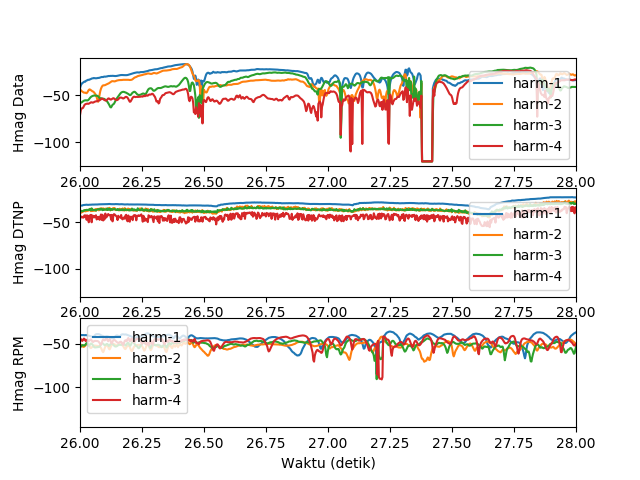
\includegraphics[width=0.8\textwidth]{resources/Analisis_wholesystem_Hmag_traindata_zoomed.png}
    \caption{(Diperbesar) Contoh magnitudo harmonik (4 harmonik pertama) yang dihasilkan oleh sistem DT-Neural Parametrik utuh dan RPM dari partitur pada data latih}\label{fig-wholesystem-hmag-output-sample-traindata-zoomed}
\end{figure}

Untuk memastikan bahwa memang arsitektur Wavenet yang dimodifikasi kurang kompleks untuk menangkap pola-pola janga-pendek yang disebutkan, dilakukan percobaan \textit{curve-fitting} data sintetik kecil. Data sintetik kecil ini bukan data pengkodean suara, namun memiliki pola-pola yang telah disebutkan. Pola-pola ini adalah \textit{spike}, osilasi, bukit-bukit/punuk-punuk, dan saling menyilang antara dua output.

\begin{figure}[htbp]
    \centering
    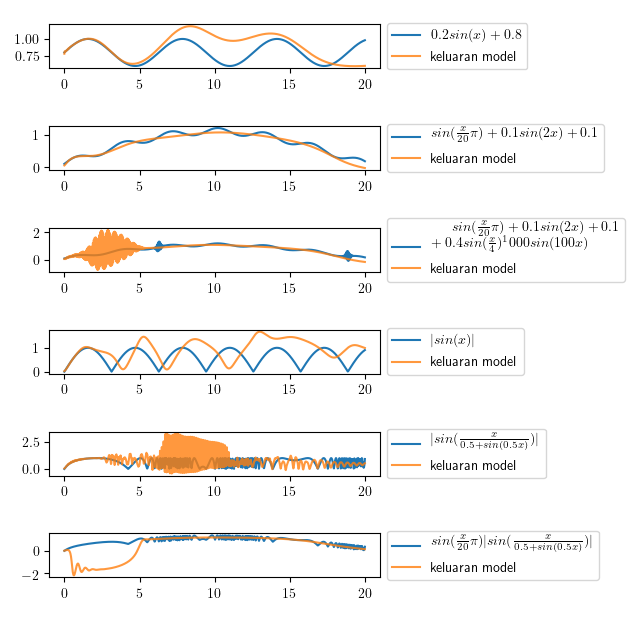
\includegraphics[width=\textwidth]{resources/analisis_modified_wavenet.png}
    \caption{Hasil percobaan \textit{curve-fitting} Wavenet yang dimodifikasi kepada data sintetik dengan satu output}\label{fig-curvefit-modified-wavenet}
\end{figure}

Gambar \ref{fig-curvefit-modified-wavenet} menunjukkan hasil \textit{curve-fitting} pola-pola detil pada satu output. Tampak bahwa apabila kurva hanya terdiri dari osilasi, jaringan syaraf tiruan Wavenet yang dimodifikasi ini dapat sedikit menangkap pola naik-turun output, meski tidak benar-benar \textit{fit} kepada kurva tersebut. Pada gambar kedua dari atas, tampak bahwa ketika pola osilasi muncul bersama pola lain yang lebih besar, pola osilasi detil menjadi hilang dan jaringan syaraf tiruan tersebut menganggap pola osilasi yang detil itu sebagai \textit{noise}.

Pada \textit{curve-fitting} pola osilasi dan pola naik turun yang besar ditambahkan dengan pola \textit{spike}, selain pola osilasi menjadi hilang, pola \textit{spike} tidak dapat ditangkap dengan benar. Muncul \textit{spike} pada saat yang tidak tepat. Pada saat yang seharusnya, \textit{spike} yang kedua tidak muncul. \textit{Spike} yang pertama muncul dengan ukuran yang jauh lebih besar daripada yang seharusnya.

Pola punuk-punuk, yang tampak pada grafik ketiga dari bawah, tidak dapat dipelajari dengan baik. Ukuran punuk berbeda dengan yang seharusnya. Bentuk pembalikan kemiringan yang tajam di bagian bawah berubah menjadi lebih halus. Setelah melewati 500 \textit{frame}, atau pada gambar ini posisi $x=10$, pola ini hilang. Pola punuk yang dipelajari semakin berbeda dari yang seharusnya ketika kerapatan punuk-punuk ini bermacam-macam.

Ketika pola punuk ini digabung dengan pola lain yang lebih besar, sebagaimana tampak pada grafik paling bawah dalam Gambar \ref{fig-curvefit-modified-wavenet}, pola punuk ini tidak ditangkap oleh jaringan syaraf tiruan ini. Yang ditangkap hanya pola umum yang lebih besar saja. Selain itu, pada bagian awal muncul keluaran yang jauh di luar \textit{range} seharusnya.

\begin{figure}[htbp]
    \centering
    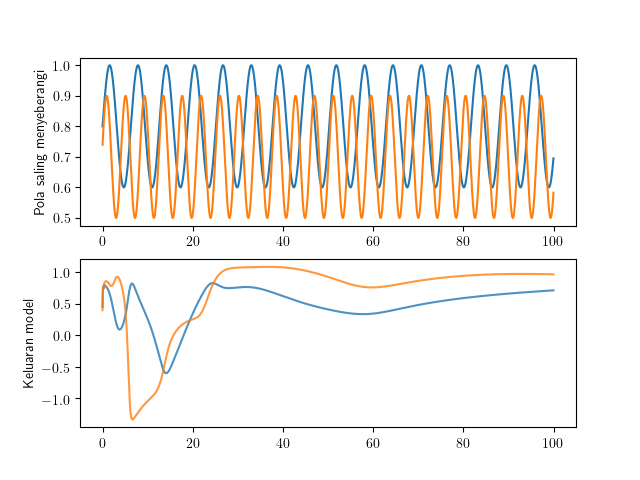
\includegraphics[width=0.8\textwidth]{resources/analisis_modified_wavenet_two_outputs.png}
    \caption{Hasil percobaan \textit{curve-fitting} Wavenet yang dimodifikasi kepada data sintetik dengan dua output}\label{fig-curvefit-modified-wavenet-two-outputs}
\end{figure}

Pola dua output yang saling menyilang terlihat pada Gambar \ref{fig-curvefit-modified-wavenet-two-outputs}. Pola ini hilang sama sekali. Memang pada bagian depan, terlihat ada saling menyilang, namun saling menyilang ini memiliki bentuk dan jarak yang berbeda dengan kurva target \textit{fitting}. Selain pada bagian depan tersebut, pada output jaringan syaraf tiruan ini tidak ada saling menyeberangi satu sama lain.

Dengan demikian, jaringan syaraf tiruan Wavenet yang dimodifikasi sebagaimana disebutkan dalam riset neural parametrik nyanyian tidak dapat mempelajari pola-pola detil yang telah disebutkan tersebut. Hal ini karena model ini kurang kompleks untuk mempelajari pola-pola detil tersebut. Akibatnya, jaringan syaraf tiruan dengan arsitektur ini tidak cocok terhadap data kode harmonik plus stokastik alat musik gesek. Jadi, kurangnya kealamian sistem secara umum dan model \textit{timbre} secara khusus disebabkan oleh tidak cocoknya arsitektur jaringan syaraf tiruan yang digunakan dengan pengkodean suara harmonik plus stokastik dan domain alat musik gesek.
